%%%%%%%%%%%%%%%%%%%%%%%%%%%%%%%%%%%%%%%%%%%%%%%%%%%%%%%%%%%%%%%%%%%%%%%%%%%%%%%%%%
\begin{frame}[fragile]\frametitle{}
\begin{center}
{\Large Numpy}

(Ref: euroscipy-numpy-tutorial)
\end{center}
\end{frame}

%%%%%%%%%%%%%%%%%%%%%%%%%%%%%%%%%%%%%%%%%%%%%%%%%%%%%%%%%%
\begin{frame}[fragile]\frametitle{A wish list}	
\begin{itemize}
  \item We want to work with vectors and matrices
 \end{itemize}

 \begin{columns}
  \begin{column}{0.55\linewidth}
   \begin{displaymath}
    \begin{pmatrix}
     a_{11} & a_{12} & \cdots & a_{1n}\\
     a_{21} & a_{22} & \cdots & a_{2n}\\
     \vdots & \vdots & \ddots & \vdots\\
     a_{n1} & a_{n2} & \cdots & a_{nn}\\
    \end{pmatrix}
   \end{displaymath}
  \end{column}%
  \begin{column}{0.45\linewidth}
   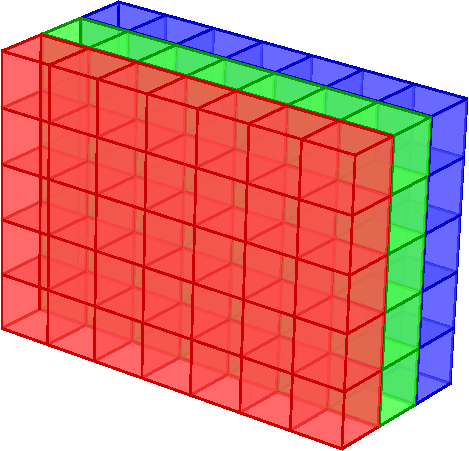
\includegraphics[width=0.7\linewidth]{rgbarray}

   colour image as $N\times M\times3$-array
  \end{column}
 \end{columns}

 \begin{itemize}
  \item we want our code to run fast
  \item we want support for linear algebra
  \item ... 
 \end{itemize}
\end{frame}

%%%%%%%%%%%%%%%%%%%%%%%%%%%%%%%%%%%%%%%%%%%%%%%%%%%%%%%%%%%%%%%%%%%%%%%%%%%%%%%%%%
\begin{frame}[fragile]\frametitle{List indexing}
 \begin{center}
  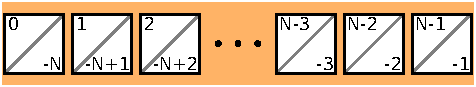
\includegraphics[width=0.96\linewidth]{listindexing2}
 \end{center}
 \begin{itemize}
  \item Indexing starts at 0
  \item Negative indices count from the end of the list to the beginning
 \end{itemize}
\end{frame}

%%%%%%%%%%%%%%%%%%%%%%%%%%%%%%%%%%%%%%%%%%%%%%%%%%%%%%%%%%%%%%%%%%%%%%%%%%%%%%%%%%
\begin{frame}[fragile]\frametitle{List slicing}

 basic syntax: \lstinline{[start:stop:step]}

 \vspace{0.2truecm}
 \begin{center}
  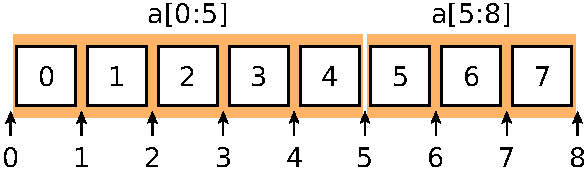
\includegraphics[width=\linewidth]{listindexing1}
 \end{center}
 \begin{itemize}
  \item if \lstinline{step=1}
  \begin{itemize}
      \item slice contains the elements \lstinline{start} to \lstinline{stop-1}
      \item slice contains \lstinline{stop-start} elements
  \end{itemize}
  \item default values:
  \begin{itemize}
      \item \makebox[1.5truecm]{\lstinline{start}\hfill} 0 (first element)
      \item \makebox[1.5truecm]{\lstinline{stop}\hfill} N-1 (last element)
      \item \makebox[1.5truecm]{\lstinline{step}\hfill} 1
  \end{itemize}
 \end{itemize}
\end{frame}

%%%%%%%%%%%%%%%%%%%%%%%%%%%%%%%%%%%%%%%%%%%%%%%%%%%%%%%%%%%%%%%%%%%%%%%%%%%%%%%%%%
\begin{frame}[fragile]\frametitle{}
 \begin{center}
  \textbf{\large\bfseries Let's do some slicing}

  \vspace{0.5truecm}
  
\includegraphics[width=3truecm]{yourturn}
 \end{center}
\end{frame}

%%%%%%%%%%%%%%%%%%%%%%%%%%%%%%%%%%%%%%%%%%%%%%%%%%%%%%%%%%%%%%%%%%%%%%%%%%%%%%%%%%
\begin{frame}[fragile, t]{Matrices and lists of lists}
 
 \vspace{0.3truecm}
 Can we use lists of lists to work with matrices?

 \begin{columns}
  \begin{column}{0.4\linewidth}
   \begin{displaymath}
    \begin{pmatrix}
     0 & 1 & 2\\
     3 & 4 & 5\\
     6 & 7 & 8
    \end{pmatrix}
   \end{displaymath}
  \end{column}%
  \begin{column}{0.6\linewidth}
   \begin{center}
    \begin{lstlisting}
matrix = [[0, 1, 2],
          [3, 4, 5],
          [6, 7, 8]]
    \end{lstlisting}

    \vspace{\baselineskip}
   \end{center}
  \end{column}
 \end{columns}
 \begin{itemize}
  \item How can we extract a row? 
  \item How can we extract a column? 
 \end{itemize}

%% \vspace{0.3truecm}
%% \begin{center}
%%  \only<2>{\textbf{\large\bfseries Let's do some experiments}
%%
%%  \vspace{0.5truecm}
%%  
\includegraphics[width=3truecm]{yourturn}}%
%%  \only<3>{\alert{Lists of lists do not work like matrices}}
%% \end{center}
\end{frame}

%%%%%%%%%%%%%%%%%%%%%%%%%%%%%%%%%%%%%%%%%%%%%%%%%%%%%%%%%%%%%%%%%%%%%%%%%%%%%%%%%%
\begin{frame}{Problems with lists as matrices}
 \begin{itemize}
  \item Different axes are not treated on equal footing
  \item Lists can contain arbitrary objects\\
        matrices have a homogeneous structure
  \item List elements can be scattered in memory
 \end{itemize}

 \vspace{0.3truecm}
 Applied to matrices \dots
 \begin{itemize}
  \item Lists are conceptually inappropriate
  \item Lists have less performance than possible
 \end{itemize}
\end{frame}

%%%%%%%%%%%%%%%%%%%%%%%%%%%%%%%%%%%%%%%%%%%%%%%%%%%%%%%%%%%%%%%%%%%%%%%%%%%%%%%%%%
\begin{frame}{We need a new object}

 \begin{center}
  \textbf{\Huge\bfseries n dimensional rray}

  \vspace{0.5truecm}
  multidimensional, homogeneous array of fixed-size items
 \end{center}
\end{frame}

%%%%%%%%%%%%%%%%%%%%%%%%%%%%%%%%%%%%%%%%%%%%%%%%%%%%%%%%%%%%%%%%%%%%%%%%%%%%%%%%%%
\begin{frame}[fragile, t]{The Wish granted!!!}
 \vspace*{-0.5truecm}
 \begin{columns}
  \begin{column}[t]{0.5\linewidth}
   \begin{center}
    \textbf{www.scipy-lectures.org}

    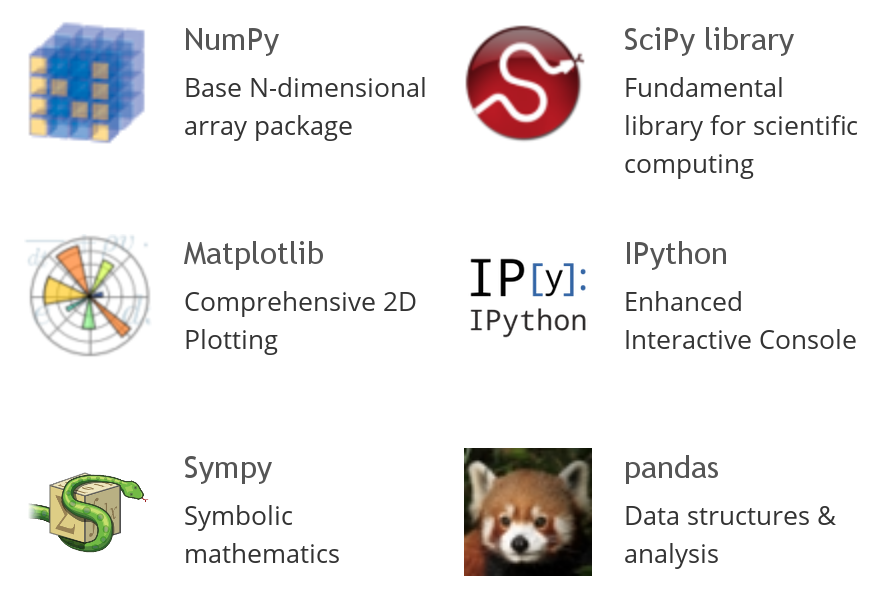
\includegraphics[width=\linewidth]{SciPyEco}
   \end{center}
  \end{column}%
  \begin{column}[t]{0.5\linewidth}
   \begin{center}
    \textbf{docs.scipy.org/doc/numpy/}

    \vspace{0.3truecm}
    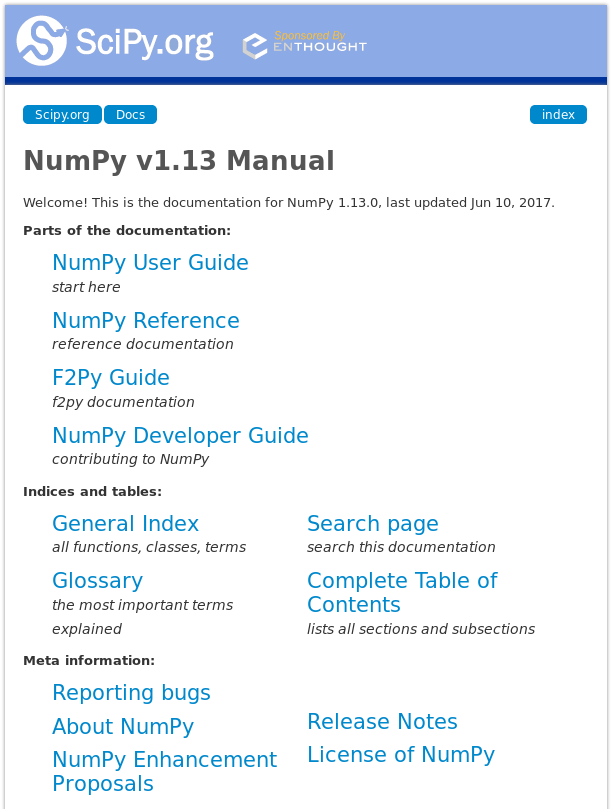
\includegraphics[width=\linewidth]{NumpyManual}
   \end{center}
  \end{column}
 \end{columns}
\end{frame}


%%%%%%%%%%%%%%%%%%%%%%%%%%%%%%%%%%%%%%%%%%%%%%%%%%%%%%%%%%%%%%%%%%%%%%%%%%%%%%%%%%
\begin{frame}[fragile, t]{Getting started}

 Import the NumPy package:
  \begin{itemize}
 \item \lstinline{from numpy import *}
 \item \lstinline{from numpy import array, sin, cos}
 \item \lstinline{import numpy}
 \item \lstinline{import numpy as np}
\end{itemize}
            \begin{center}
             
\includegraphics[width=3truecm]{yourturn}
            \end{center}
\end{frame}
%%
%%%%%%%%%%%%%%%%%%%%%%%%%%%%%%%%%%%%%%%%%%%%%%%%%%%%%%%%%%%%%%%%%%%%%%%%%%%%%%%%%%%%
%%\begin{frame}[fragile]\frametitle{Data types}
%%Some important data types:
%%\begin{tabular}{ll}
%%integer & \lstinline{int8}, \lstinline{int16}, \lstinline{int32}, \lstinline{int64}, \lstinline{uint8}, ...\\
%%float   & \lstinline{float16}, \lstinline{float32}, \lstinline{float64}, ... \\
%%complex & \lstinline{complex64}, \lstinline{complex128}, ...\\
%%boolean & \lstinline{bool8}\\
%%Unicode string  & \\
%%\end{tabular}
%%
%%Default: Python float
%%%\begin{center}
%%% \alert{\raisebox{0.4em}{}\quad Beware of overflows!}
%%%\end{center}
%%%\begin{center}
%%% 
\includegraphics[width=3truecm]{yourturn}
%%%\end{center}
%%\end{frame}

%%%%%%%%%%%%%%%%%%%%%%%%%%%%%%%%%%%%%%%%%%%%%%%%%%%%%%%%%%%%%%%%%%%%%%%%%%%%%%%%%%
\begin{frame}[fragile]\frametitle{Strides}
 \begin{columns}
  \begin{column}{0.33\linewidth}
   \begin{displaymath}
    \begin{pmatrix}
     0 & 1 & 2 & 3 & 4 & 5
    \end{pmatrix}
   \end{displaymath}
  \end{column}%
  \begin{column}{0.67\linewidth}
   (8,)

   \vspace{0.2truecm}
   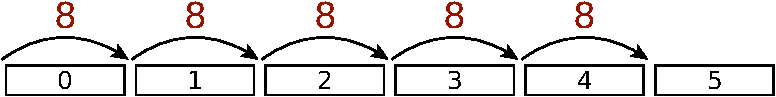
\includegraphics[width=0.8\linewidth]{strides_0}
  \end{column}
 \end{columns}

 \vspace{0.8truecm}
 \begin{columns}
  \begin{column}{0.33\linewidth}
   \begin{displaymath}
    \begin{pmatrix}
     0 & 1 & 2\\
     3 & 4 & 5
    \end{pmatrix}
   \end{displaymath}
  \end{column}%
  \begin{column}{0.67\linewidth}
   (24, 8)

   \vspace{0.2truecm}
   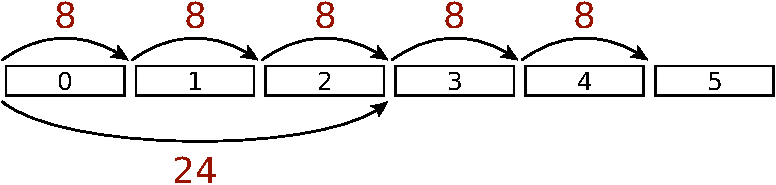
\includegraphics[width=0.8\linewidth]{strides_3}
  \end{column}
 \end{columns}

 \vspace{0.8truecm}
 \begin{columns}
  \begin{column}{0.33\linewidth}
   \begin{displaymath}
    \begin{pmatrix}
     0 & 1 \\
     2 & 3 \\
     4 & 5
    \end{pmatrix}
   \end{displaymath}
  \end{column}%
  \begin{column}{0.67\linewidth}
   (16, 8)

   \vspace{0.2truecm}
   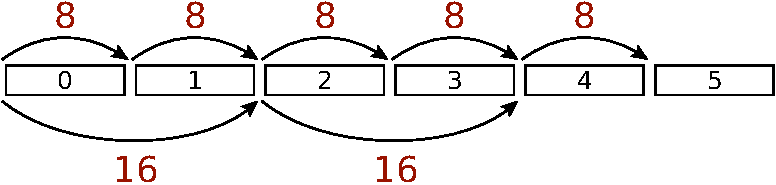
\includegraphics[width=0.8\linewidth]{strides_2}
  \end{column}
 \end{columns}
\end{frame}

%%%%%%%%%%%%%%%%%%%%%%%%%%%%%%%%%%%%%%%%%%%%%%%%%%%%%%%%%%%%%%%%%%%%%%%%%%%%%%%%%%
\begin{frame}[fragile]\frametitle{Views}
 For the sake of efficiency, NumPy uses views if possible.

 \begin{itemize}
  \item Changing one or more matrix elements will change it in all views.
  \item Example: transposition of a matrix \lstinline{a.T}\\
        No need to copy the matrix and to create a new one
 \end{itemize}

% \begin{center}
%  
\includegraphics[width=3truecm]{yourturn}
% \end{center}
\end{frame}

%%%%%%%%%%%%%%%%%%%%%%%%%%%%%%%%%%%%%%%%%%%%%%%%%%%%%%%%%%%%%%%%%%%%%%%%%%%%%%%%
\begin{frame}[fragile]\frametitle{Some array creation routines}

 \begin{itemize}
  \item numerical ranges:
        \lstinline{arange}, \lstinline{linspace}, \lstinline{logspace}
  \item homogeneous data:
        \lstinline{zeros}, \lstinline{ones}
  \item diagonal elements:
        \lstinline{diag}, \lstinline{eye}
  \item random numbers:
        \lstinline{rand}, \lstinline{randint}
 \end{itemize}

 \vspace{0.3truecm}
 \begin{columns}
  \begin{column}{0.02\linewidth}
   \alert{\raisebox{1.0em}{}}
  \end{column}%
  \begin{column}{0.98\linewidth}
   \alert{Numpy has an \lstinline{append()}-method. Avoid it if possible.}
  \end{column}
 \end{columns}

 \vspace{0.3truecm}
% \begin{center}
%  
\includegraphics[width=3truecm]{yourturn}
% \end{center}
\end{frame}

%%%%%%%%%%%%%%%%%%%%%%%%%%%%%%%%%%%%%%%%%%%%%%%%%%%%%%%%%%%%%%%%%%%%%%%%%%%%%%%
\begin{frame}[fragile]\frametitle{Indexing and slicing in one dimension}
 \textbf{1d arrays}: indexing and slicing as for lists

 \begin{itemize}
  \item first element has index 0
  \item negative indices count from the end
  \item slices: \lstinline{[start:stop:step]}\\
        \strut\hphantom{slices:\ }  without the element indexed by \lstinline{stop}
  \item if values are omitted:
        \begin{itemize}
         \item \lstinline{start}: starting from first element
         \item \lstinline{stop}: until (and including) the last element
         \item \lstinline{step}: all elements between \lstinline{start} and \lstinline{stop}-1
        \end{itemize}
 \end{itemize}

%% \begin{center}
%%  
\includegraphics[width=3truecm]{yourturn}
%% \end{center}
\end{frame}

%%%%%%%%%%%%%%%%%%%%%%%%%%%%%%%%%%%%%%%%%%%%%%%%%%%%%%%%%%%%%%%%%%%%%%%%%%%%%%%
\begin{frame}[fragile]\frametitle{Indexing and slicing in higher dimensions}
 \begin{itemize}
  \item usual slicing syntax
  \item difference to lists:\\
        slices for the various axes separated by comma
 \end{itemize}

 \begin{center}
  \only<1>{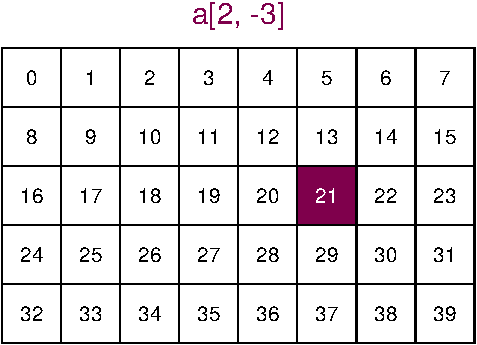
\includegraphics[width=0.8\linewidth]{arraygraphics_0}}%
  \only<2>{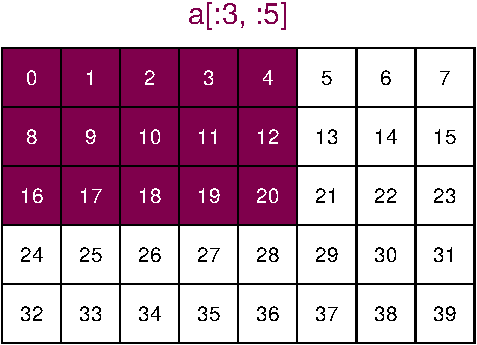
\includegraphics[width=0.6\linewidth]{arraygraphics_1}}
 \end{center}
\end{frame}

%%%%%%%%%%%%%%%%%%%%%%%%%%%%%%%%%%%%%%%%%%%%%%%%%%%%%%%%%%%%%%%%%%%%%%%%%%%%%%%
\begin{frame}[fragile]\frametitle{Indexing and slicing in higher dimensions}
% \begin{center}
%  
\includegraphics[width=3truecm]{yourturn}
% \end{center}

 \begin{center}
  \only<1>{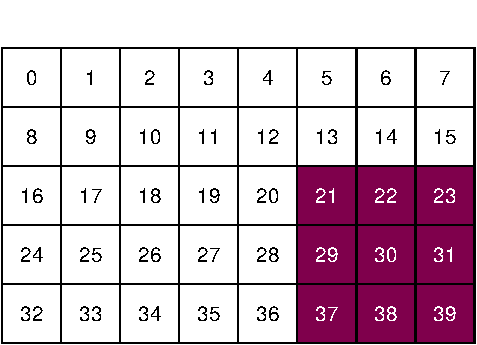
\includegraphics[width=0.6\linewidth]{arraygraphics_2_wo}}%
  \only<2>{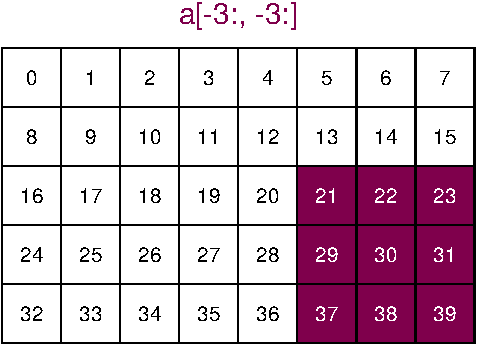
\includegraphics[width=0.6\linewidth]{arraygraphics_2}}%
  \only<3>{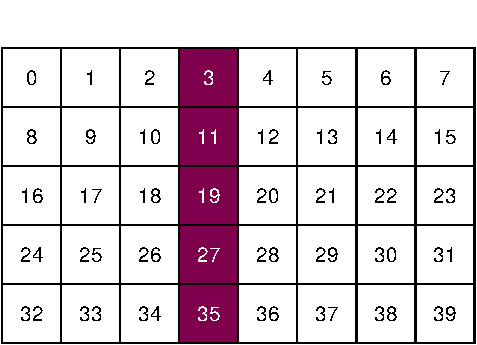
\includegraphics[width=0.6\linewidth]{arraygraphics_3_wo}}%
  \only<4>{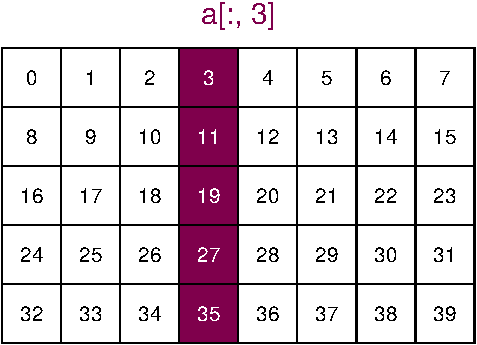
\includegraphics[width=0.6\linewidth]{arraygraphics_3}}%
  \only<5>{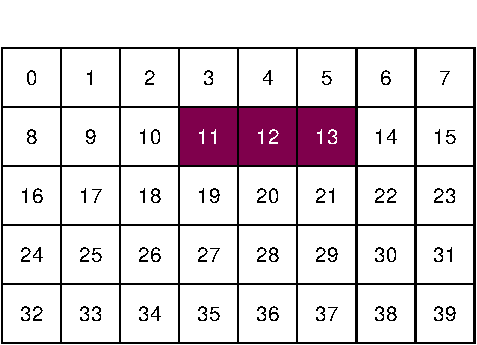
\includegraphics[width=0.6\linewidth]{arraygraphics_4_wo}}%
  \only<6>{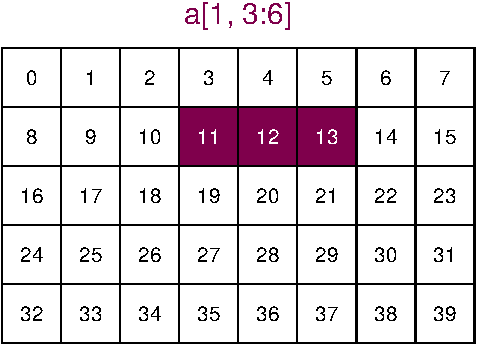
\includegraphics[width=0.6\linewidth]{arraygraphics_4}}%
  \only<7>{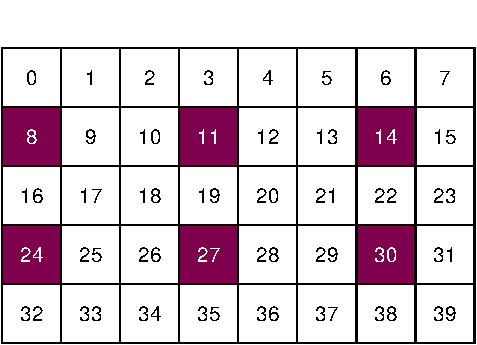
\includegraphics[width=0.6\linewidth]{arraygraphics_5_wo}}%
  \only<8>{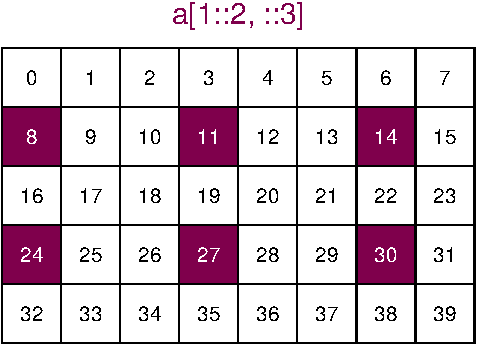
\includegraphics[width=0.6\linewidth]{arraygraphics_5}}
 \end{center}
\end{frame}

%%%%%%%%%%%%%%%%%%%%%%%%%%%%%%%%%%%%%%%%%%%%%%%%%%%%%%%%%%%%%%%%%%%%%%%%%%%%%%%
\begin{frame}{Fancy indexing -- Boolean mask}
 \begin{center}
  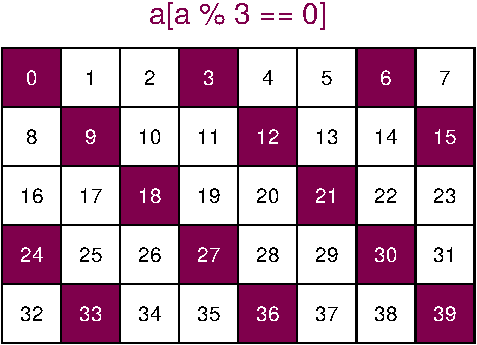
\includegraphics[width=0.8\linewidth]{arraygraphics_6}
 \end{center}
\end{frame}

\begin{frame}{Fancy indexing -- array of integers}
 \begin{center}
  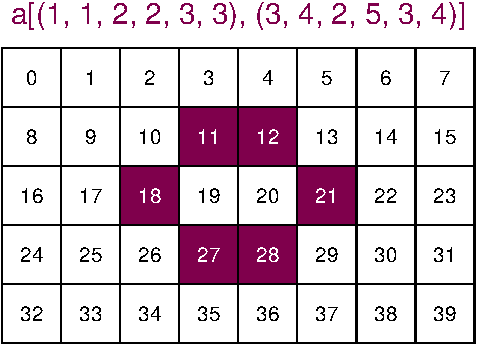
\includegraphics[width=0.8\linewidth]{arraygraphics_7}
 \end{center}
\end{frame}

%%%%%%%%%%%%%%%%%%%%%%%%%%%%%%%%%%%%%%%%%%%%%%%%%%%%%%%%%%%%%%%%%%%%%%%%%%%%%%%%%
%%\begin{frame}{Application: sieve of Eratosthenes}
%% 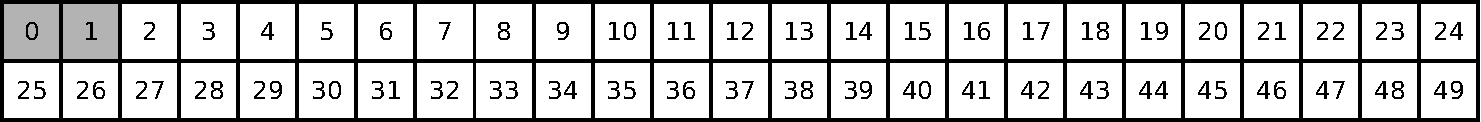
\includegraphics[width=\linewidth]{eratosthenes_1}\\[0.3truecm]
%% 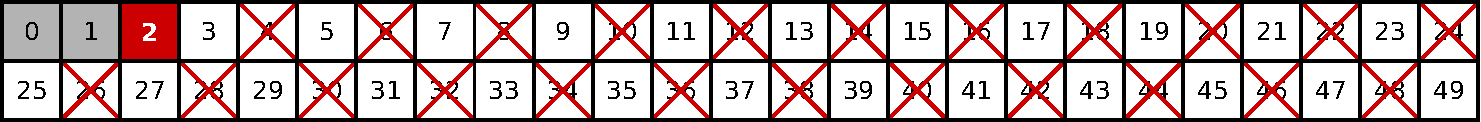
\includegraphics[width=\linewidth]{eratosthenes_2}\\[0.3truecm]
%% 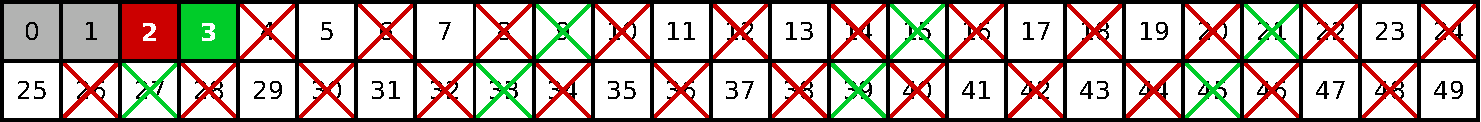
\includegraphics[width=\linewidth]{eratosthenes_3}\\[0.3truecm]
%% 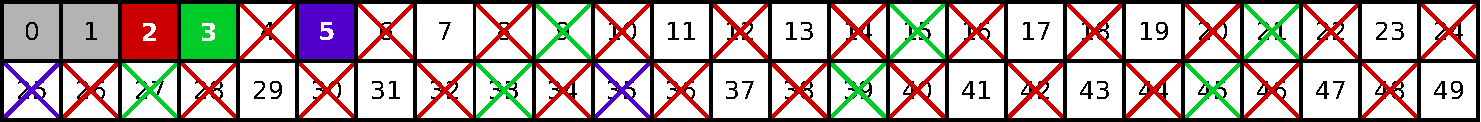
\includegraphics[width=\linewidth]{eratosthenes_4}\\[0.3truecm]
%% 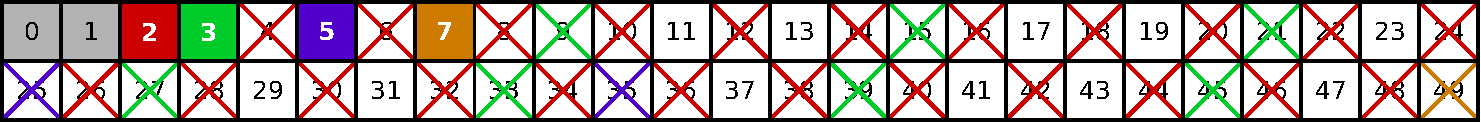
\includegraphics[width=\linewidth]{eratosthenes_5}\\[0.3truecm]
%% 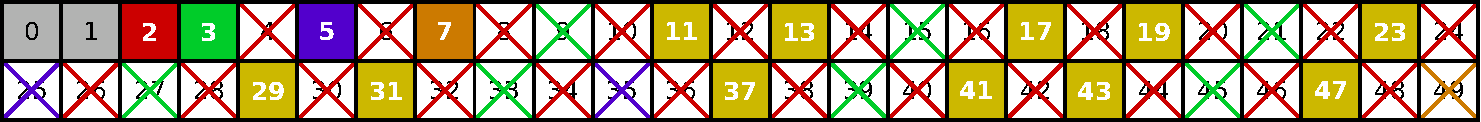
\includegraphics[width=\linewidth]{eratosthenes_6}
%%\end{frame}

%%%%%%%%%%%%%%%%%%%%%%%%%%%%%%%%%%%%%%%%%%%%%%%%%%%%%%%%%%%%%%%%%%%%%%%%%%%%%%%
\begin{frame}{Axes}
 \begin{Large}
  \begin{displaymath}
   \begin{pmatrix}
    a_{11} & a_{12} & a_{13} \\
    a_{21} & a_{22} & a_{23} \\
    a_{31} & a_{32} & a_{33} \\
   \end{pmatrix}
  \end{displaymath}
 \end{Large}

 \begin{center}
  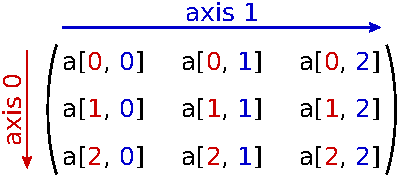
\includegraphics[width=0.7\linewidth]{axes}
 \end{center}

 \begin{columns}
  \begin{column}{0.4\linewidth}
%   \begin{center}
%    
\includegraphics[width=3truecm]{yourturn}
%   \end{center}
  \end{column}%
  \begin{column}{0.6\linewidth}
   np.sum(a)\\
   np.sum(a, axis=$...$)
  \end{column}
 \end{columns}
\end{frame}

%%%%%%%%%%%%%%%%%%%%%%%%%%%%%%%%%%%%%%%%%%%%%%%%%%%%%%%%%%%%%%%%%%%%%%%%%%%%
\begin{frame}[fragile]{Axes in more than two dimensions}
 \begin{columns}
  \begin{column}{0.4\linewidth}
   \begin{center}
   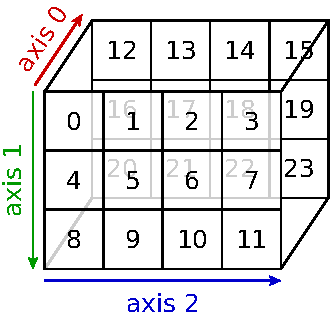
\includegraphics[width=0.95\linewidth]{array3d}
   \end{center}
  \end{column}%
  \begin{column}{0.6\linewidth}
   \begin{verbatim}
array(/\textcolor{myred}{[}\textcolor{mygreen}{[}\textcolor{myblue}{[}/ 0,  1,  2,  3/\textcolor{myblue}{]}/,
        /\textcolor{myblue}{[}/ 4,  5,  6,  7/\textcolor{myblue}{]}/,
        /\textcolor{myblue}{[}/ 8,  9, 10, 11/\textcolor{myblue}{]}\textcolor{mygreen}{]}/,

       /\textcolor{mygreen}{[}\textcolor{myblue}{[}/12, 13, 14, 15/\textcolor{myblue}{]}/,
        /\textcolor{myblue}{[}/16, 17, 18, 19/\textcolor{myblue}{]}/,
        /\textcolor{myblue}{[}/20, 21, 22, 23/\textcolor{myblue}{]}\textcolor{mygreen}{]}\textcolor{myred}{]}/)
    \end{verbatim}%
  \end{column}
 \end{columns}

 \vspace{0.5truecm}
 \begin{columns}
  \begin{column}{0.3\linewidth}
%   \begin{center}
%    
\includegraphics[width=3truecm]{yourturn}
%   \end{center}
  \end{column}%
  \begin{column}{0.6\linewidth}
   Create this array and produce 2d arrays by cutting perpendicular to the axes 0, 1, and 2
  \end{column}
 \end{columns}
\end{frame}

%%%%%%%%%%%%%%%%%%%%%%%%%%%%%%%%%%%%%%%%%%%%%%%%%%%%%%%%%%%%%%%%%%%%%%%%%%%%
\begin{frame}[fragile]{Matrix multiplication}
 \begin{columns}
  \begin{column}{0.6\linewidth}
   \begin{center}
    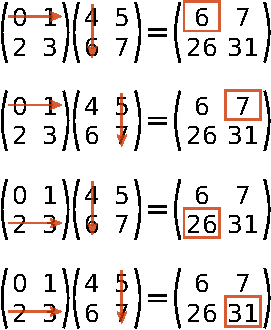
\includegraphics[width=0.8\linewidth]{matrixmult}
   \end{center}
  \end{column}%
  \begin{column}{0.4\linewidth}
%   
\includegraphics[width=3truecm]{yourturn}

   \vspace{0.4truecm}
   try \lstinline{np.dot$(\bullet, \bullet)$}\\
   \strut\hphantom{try\ }\lstinline{\bullet.dot(\bullet)}\\
   \strut\hphantom{try\ }\lstinline{$\bullet\,@\,\bullet$}\,$^{*)}$
   
   \vspace{0.7truecm}
   \hbox to 1truecm{\hrulefill}
   \scriptsize{$^{*)}$ Python$\geq$3.5, NumPy$\geq$1.10}
   \vspace{1truecm}
  \end{column}
 \end{columns}
\end{frame}


%%%%%%%%%%%%%%%%%%%%%%%%%%%%%%%%%%%%%%%%%%%%%%%%%%%%%%%%%%%%%%%%%%%%%%%%%
\begin{frame}[fragile]\frametitle{Mathematical functions in NumPy}
 \hspace*{-0.45truecm} Universal functions (ufuncs) take ndarrays as argument

 \vspace{0.4truecm}
 \begin{columns}[t]
  \begin{column}{0.5\linewidth}
   \begin{scriptsize}%
    \textbf{Trigonometric functions}\\
     {\tiny sin, cos, tan, arcsin, arccos, arctan, hypot, arctan2, degrees,
      radians, unwrap, deg2rad, rad2deg}\\[0.2truecm]
   \textbf{Hyperbolic functions}\\
     {\tiny sinh, cosh, tanh, arcsinh, arccosh, arctanh}\\[0.2truecm]
   \textbf{Rounding}\\
     {\tiny around, round\_, rint, fix, floor, ceil, trunc}\\[0.2truecm]
   \textbf{Sums, products, differences}\\
     {\tiny prod, sum, nansum, cumprod, cumsum, diff, ediff1d,
      gradient, cross, trapz}\\[0.2truecm]
   \textbf{Exponents and logarithms}\\
     {\tiny exp, expm1, exp2, log, log10, log2, log1p, logaddexp,
      logaddexp2}\\[0.2truecm]
   \end{scriptsize}
  \end{column}%
  \begin{column}{0.5\linewidth}
   \begin{scriptsize}%
    \textbf{Other special functions}\\
     {\tiny i0, sinc}\\[0.2truecm]
    \textbf{Floating point routines}\\
     {\tiny signbit, copysign, frexp, ldexp}\\[0.2truecm]
    \textbf{Arithmetic operations}\\
     {\tiny add, reciprocal, negative, multiply, divide, power, subtract,
      true\_divide, floor\_divide, fmod, mod, modf, remainder}\\[0.2truecm]
    \textbf{Handling complex numbers}\\
     {\tiny angle, real, imag, conj}\\[0.2truecm]
    \textbf{Miscellaneous}\\
     {\tiny convolve, clip, sqrt, square, absolute, fabs, sign, maximum,
      minimum, fmax, fmin, nan\_to\_num, real\_if\_close, interp}\\
   \end{scriptsize}
  \end{column}
 \end{columns}

 \vspace{0.5truecm}
 \hspace*{-0.32truecm}{\small Many more special functions are provided as ufuncs by SciPy}
\end{frame}

%%%%%%%%%%%%%%%%%%%%%%%%%%%%%%%%%%%%%%%%%%%%%%%%%%%%%%%%%%%%%%%%%%%%%%%%%
\begin{frame}[fragile]\frametitle{Rules for broadcasting}
 Arrays can be broadcast to the same shape if one of the following points is
 fulfilled:
 \begin{enumerate}
  \item The arrays all have exactly the same shape.
  \item The arrays all have the same number of dimensions and the
        length of each dimension is either a common length or 1.
  \item The arrays that have too few dimensions can have their
        shapes prepended with a dimension of length 1 to satisfy
        property 2.
 \end{enumerate}
\end{frame}

%%%%%%%%%%%%%%%%%%%%%%%%%%%%%%%%%%%%%%%%%%%%%%%%%%%%%%%%%%%%%%%%%%%%%%%%%
\begin{frame}[fragile]\frametitle{Broadcasting}
 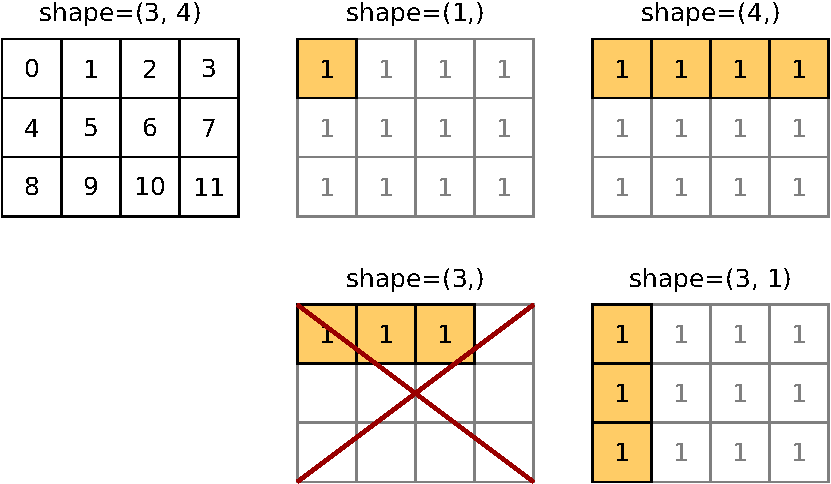
\includegraphics[width=\linewidth]{broadcast}

% \vspace{-0.3truecm}
%  
\includegraphics[width=3truecm]{yourturn}
\end{frame}

\begin{frame}{Application: Mandelbrot set}
 \begin{displaymath}
  z_{n+1} = z_n^2+c,\ \ z_0=0
 \end{displaymath}

 Mandelbrot set contains the points for which $z$ remains bounded.

 \begin{columns}
  \begin{column}{0.5\linewidth}
   \begin{center}
    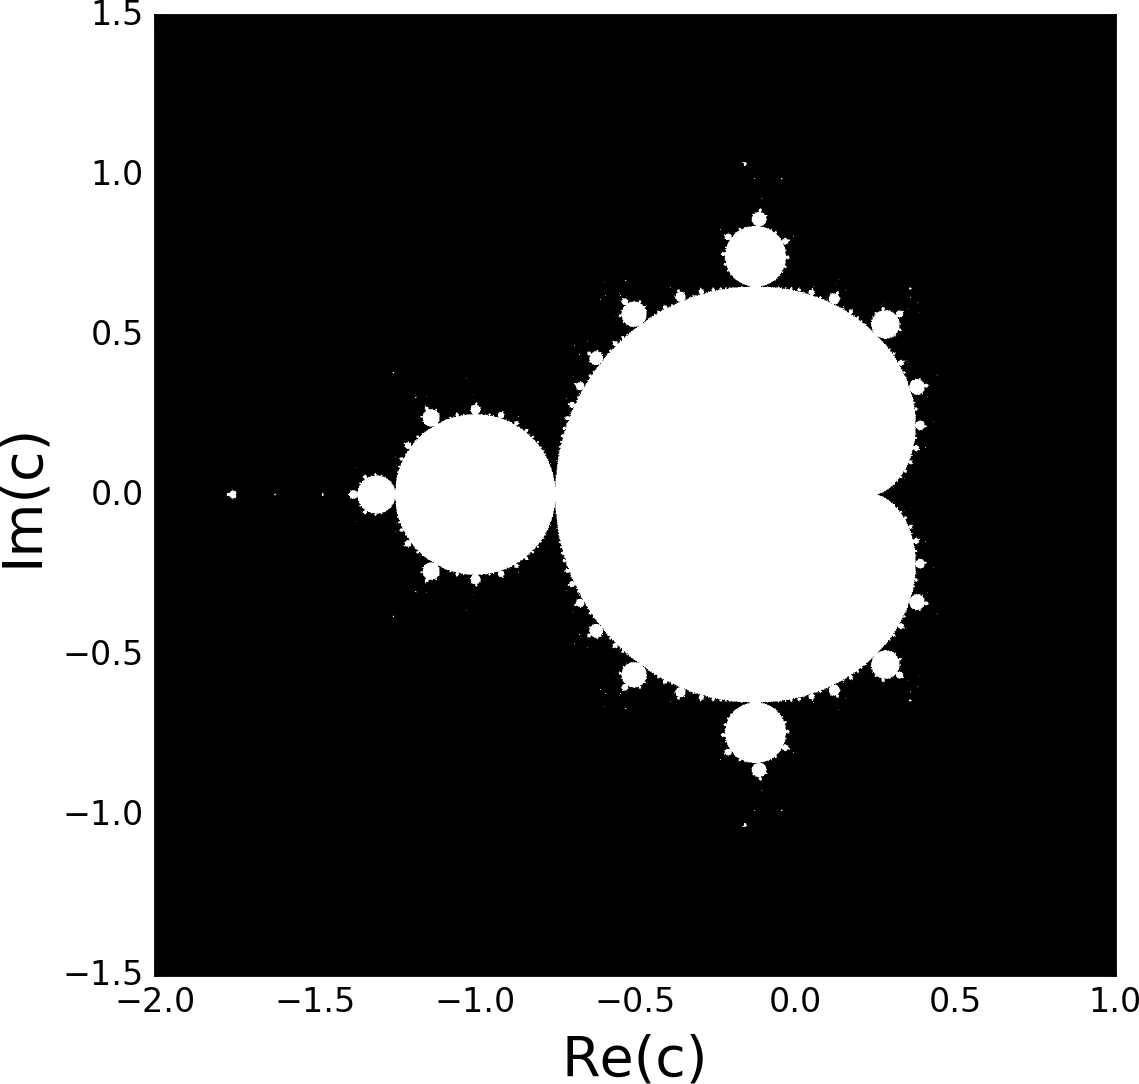
\includegraphics[width=0.8\linewidth]{mandelbrot}

    \vspace{0.3truecm}
%    
\includegraphics[width=3truecm]{yourturn}
   \end{center}
  \end{column}%
  \begin{column}{0.5\linewidth}
   \begin{center}
    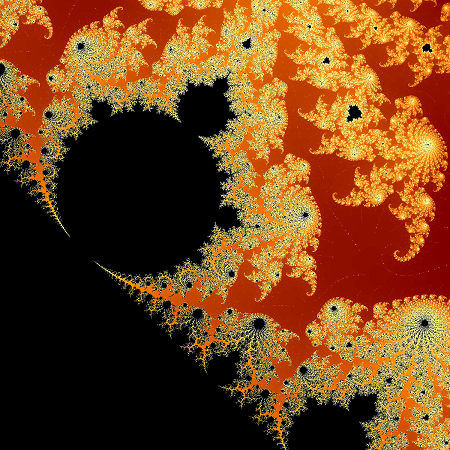
\includegraphics[width=0.675\linewidth]{mandelbrot_detail}

    \vspace{2.35truecm}
   \end{center}
  \end{column}
 \end{columns}
\end{frame}

%%%%%%%%%%%%%%%%%%%%%%%%%%%%%%%%%%%%%%%%%%%%%%%%%%%%%%%%%%%%%%%%%%%%%%
\begin{frame}[fragile]\frametitle{Application: $\pi$ from random numbers}
 \begin{columns}
  \begin{column}{0.4\linewidth}
   \begin{center}
    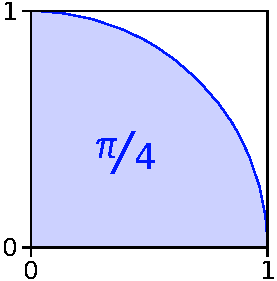
\includegraphics[width=0.8\linewidth]{random_pi}
   \end{center}
  \end{column}%
  \begin{column}{0.6\linewidth}
   \begin{enumerate}
    \item Create pairs of random numbers and determine the fraction of pairs which
          has a distance from the origin less than one.
    \item Multiply the result by four to obtain an approximation of $\pi$.
   \end{enumerate}
  \end{column}
 \end{columns}

 \vspace{0.5truecm}
 hint: \lstinline{count\_nonzero(a)} counts the number of non-zero values in the array \lstinline{a} and
 also works for Boolean arrays. Remember that \lstinline{np.info()} can be helpful.

% \vspace{0.3truecm}
% \begin{center}
%  
\includegraphics[width=3truecm]{yourturn}
% \end{center}
\end{frame}

%%%%%%%%%%%%%%%%%%%%%%%%%%%%%%%%%%%%%%%%%%%%%%%%%%%%%%%%%%%%%%%%%%%%%%
\begin{frame}[fragile]\frametitle{Fibonacci series and linear algebra}
 \begin{center}
  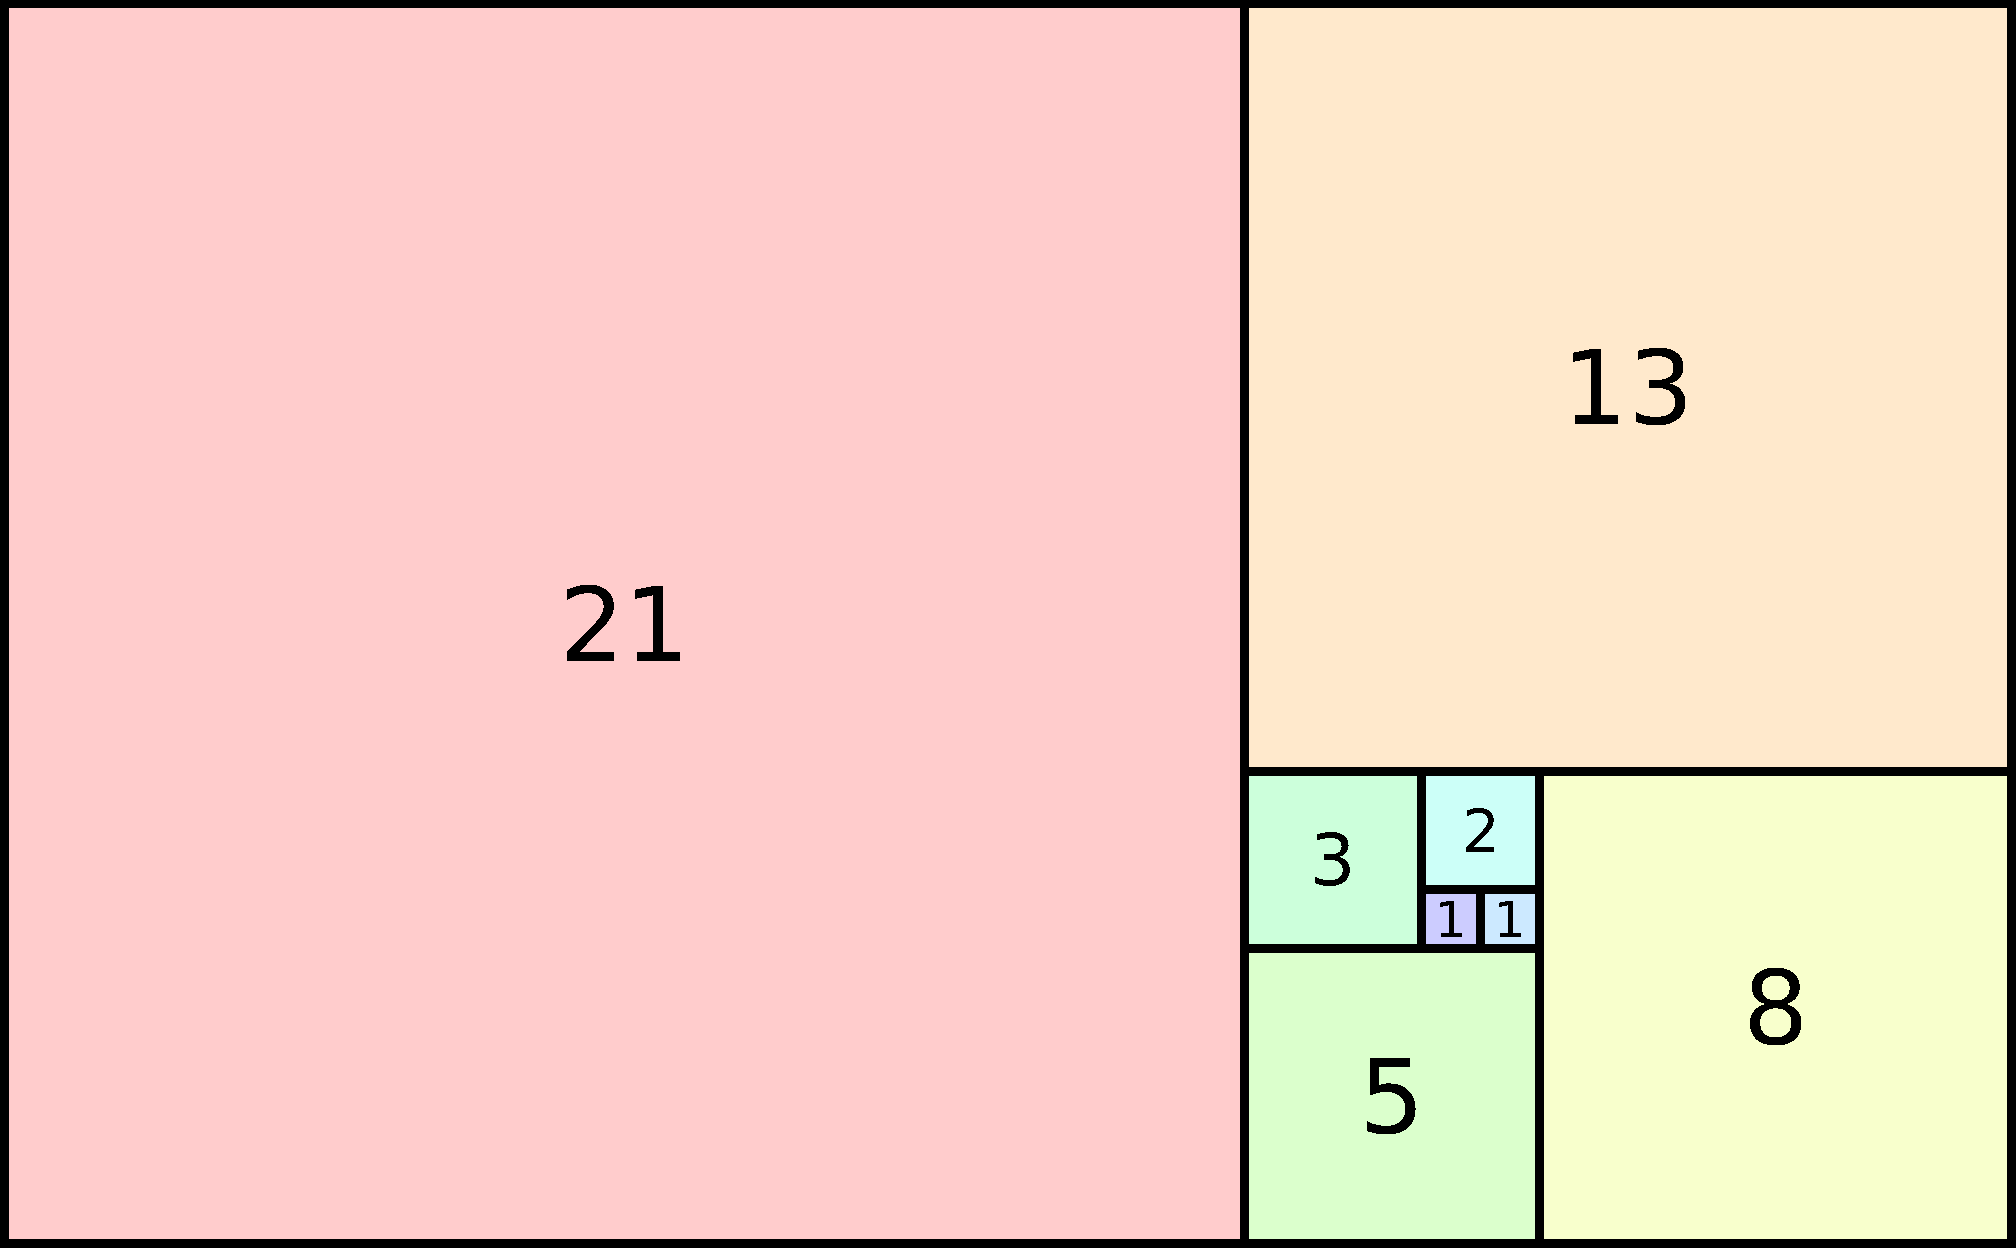
\includegraphics[width=0.7\linewidth]{fibonacci}
 \end{center}

 \vspace{-0.3truecm}
 \begin{columns}[c]
  \begin{column}{0.5\linewidth}
   Fibonacci series:\\ 1, 1, 2, 3, 5, 8, 13, 21, ...
  \end{column}%
  \begin{column}{0.5\linewidth}
   \begin{displaymath}
    F_{n+1} = F_n + F_{n-1},\quad F_1 = F_2 = 1
   \end{displaymath}

   \vspace{-0.8truecm}
   \begin{displaymath}
    \strut\quad\mathrm{or:}\quad
    \begin{pmatrix} 1 & 1 \\ 1 & 0 \end{pmatrix} 
    \begin{pmatrix} F_n \\ F_{n-1} \end{pmatrix} =
    \begin{pmatrix} F_{n+1} \\ F_n \end{pmatrix}
   \end{displaymath}
  \end{column}
 \end{columns}

 \begin{center}
  What is the limit of $F_{n+1}/F_n$ for large $n$?
 \end{center}
\end{frame}

%%%%%%%%%%%%%%%%%%%%%%%%%%%%%%%%%%%%%%%%%%%%%%%%%%%%%%%%%%%%%%%%%%%%%%
\begin{frame}[fragile]\frametitle{Eigenvalue problems}
 \begin{displaymath}
  \begin{pmatrix}
   a_{11} & \cdots & a_{1n} \\
   \vdots & \ddots & \vdots \\
   a_{n1} & \cdots & a_{nn}
  \end{pmatrix}\begin{pmatrix}
   v_1^{(k)} \\ \vdots \\ v_n^{(k)}
  \end{pmatrix} = \lambda^{(k)}
  \begin{pmatrix}
   v_1^{(k)} \\ \vdots \\ v_n^{(k)}
  \end{pmatrix}\qquad k=1,..., n
 \end{displaymath}

 \begin{center}
  eigenvalue $\lambda^{(k)}$\qquad\qquad
  eigenvector $\begin{pmatrix}v_1^{(k)}\\\vdots\\v_n^{(k)}\end{pmatrix}$
 \end{center}

 for our Fibonacci problem:
   \begin{displaymath}
    \begin{pmatrix} 1 & 1 \\ 1 & 0 \end{pmatrix} 
    \begin{pmatrix} F_n \\ F_{n-1} \end{pmatrix} =
    \alert{\lambda}\begin{pmatrix} F_{n+1} \\ F_n \end{pmatrix}
   \end{displaymath}

 We are looking for the eigenvalue larger than one.
\end{frame}

%%%%%%%%%%%%%%%%%%%%%%%%%%%%%%%%%%%%%%%%%%%%%%%%%%%%%%%%%%%%%%%%%%%%%%
\begin{frame}[fragile]\frametitle{Linear algebra in NumPy}
 \lstinline{import numpy.linalg as LA}


 \textbf{Matrix and vector products}\\
 {\small dot, vdot, inner, outer, matmul, tensordot, einsum, LA.matrix\_power,
 kron}\\[0.2truecm]
 
 \textbf{Decompositions}\\
 {\small LA.cholesky, LA.qr, LA.svd}\\
 
 \textbf{Matrix eigenvalues}\\
 
 \alert{\small LA.eig, LA.eigh, LA.eigvals, LA.eigvalsh}\qquad
% 
\includegraphics[width=3truecm]{yourturn}\\[0.2truecm]

 \textbf{Norms and other numbers}\\
 {\small LA.norm, LA.cond, LA.det, LA.matrix\_rank, LA.slogdet,
 trace}\\[0.2truecm]
 
 \textbf{Solving equations and inverting matrices}
 {\small LA.solve, LA.tensorsolve, LA.lstsq, LA.inv, LA.pinv, LA.tensorinv}

 \vspace{0.6truecm}
 hint: see also the methods for linear algebra in SciPy
\end{frame}

%%%%%%%%%%%%%%%%%%%%%%%%%%%%%%%%%%%%%%%%%%%%%%%%%%%%%%%%%%%%%%%%%%%
\begin{frame}{Statistics in NumPy}
 \textbf{Order statistics}\\
 \small{amin, amax, nanmin, nanmax, ptp, percentile, nanpercentile}\\[0.2truecm]
 \textbf{Averages and variances}\\
 \small{median, average, mean, std, var, nanmedian, nanmean, nanstd, nanvar}\\[0.2truecm]
 \textbf{Correlating}\\
 \small{corrcoef, correlate, cov}\\[0.2truecm]
 \textbf{Histograms}\\
 \small{histogram, histogram2d, histogramdd, bincount, digitize}
\end{frame}

%%%%%%%%%%%%%%%%%%%%%%%%%%%%%%%%%%%%%%%%%%%%%%%%%%%%%%%%%%%%%%%%%%%
\begin{frame}{Application: Brownian motion}
 \begin{center}
  
\includegraphics[width=0.8\linewidth]{diffusion}
 \end{center}

 \begin{enumerate}
  \item Simulate several trajectories for a one-dimensional Brownian motion\\
        hint: \lstinline{np.random.choice}
  \item Plot the mean distance from the origin as a function of time\\
  \item Plot the variance of the trajectories as a function of time
 \end{enumerate}

% \vspace{0.3truecm}
% \begin{center}
%  \includegraphics[width=3truecm]{yourturn}
% \end{center}
\end{frame}

%%%%%%%%%%%%%%%%%%%%%%%%%%%%%%%%%%%%%%%%%%%%%%%%%%%%%%%%%%%%%%%%%%%
\begin{frame}[fragile]\frametitle{Sorting, searching, and counting in NumPy}
 
 \textbf{Sorting}\\
 \small{sort, lexsort, argsort, ndarray.sort, msort, sort\_complex, partition,
        argpartition}\\[0.2truecm]
 \textbf{Searching}\\
 \small{argmax, nanargmax, argmin, nanargmin, argwhere, nonzero, flatnonzero,
        where, searchsorted, extract}\\[0.2truecm]
 \textbf{Counting}\\
 \small{count\_nonzero}
\end{frame}

%%%%%%%%%%%%%%%%%%%%%%%%%%%%%%%%%%%%%%%%%%%%%%%%%%%%%%%%%%%%%%%%%%%
\begin{frame}{Application: identify entry closest to $\frac{1}{2}$}
 \begin{displaymath}
  \begin{pmatrix}
   0.05344164 & \alert{0.37648768} & 0.80691163 & 0.71400815\\
   \alert{0.60825034} & 0.35778938 & 0.37393356 & 0.32615374\\
   0.83118547 & 0.33178711 & 0.21548027 & \alert{0.42209291}
  \end{pmatrix}
 \end{displaymath}

 \begin{displaymath}
  \Downarrow
 \end{displaymath}

 \begin{displaymath}
  \begin{pmatrix}
   \alert{0.37648768}\\ \alert{0.60825034}\\ \alert{0.42209291}
  \end{pmatrix}
 \end{displaymath}

 \vspace{0.3truecm}
% \includegraphics[width=3truecm]{yourturn}\qquad
 \raisebox{0.7truecm}{hint: use \lstinline{np.argsort}}
\end{frame}

%%%%%%%%%%%%%%%%%%%%%%%%%%%%%%%%%%%%%%%%%%%%%%%%%%%%%%%%%%%%%%%%%%%
\begin{frame}[fragile]\frametitle{Polynomials in NumPy}
 Power series: \lstinline{numpy.polynomial.polynomial}

 \vspace{0.2truecm}
 \textbf{Polynomial Class}\\
 \small{Polynomial}\\[0.1truecm]
 \textbf{Basics}\\
 \small{polyval, polyval2d, polyval3d, polygrid2d, polygrid3d, polyroots,
        polyfromroots}\\[0.1truecm]
 \textbf{Fitting}\\
 \small{polyfit, polyvander, polyvander2d, polyvander3d}\\[0.1truecm]
 \textbf{Calculus}\\
 \small{polyder, polyint}\\[0.1truecm]
 \textbf{Algebra}\\
 \small{polyadd, polysub, polymul, polymulx, polydiv, polypow}\\[0.1truecm]
 \textbf{Miscellaneous}\\
 \small{polycompanion, polydomain, polyzero, polyone, polyx, polytrim, polyline}

 \vspace{0.2truecm}
 \small{also: Chebyshev, Legendre, Laguerre, Hermite polynomials}
\end{frame}

%%%%%%%%%%%%%%%%%%%%%%%%%%%%%%%%%%%%%%%%%%%%%%%%%%%%%%%%%%%%%%%%%%%
\begin{frame}[fragile]\frametitle{Some examples}
 \begin{small}
  \textbf{\lstinline{P.Polynomial([24, -50, 35, -10, 1])}}
  \begin{displaymath}
   p_4(x) = x^4-10x^3+35x^2-50x+24 = (x-1)(x-2)(x-3)(x-4)
  \end{displaymath}

  \textbf{\lstinline{p4.deriv()}}
  \begin{displaymath}
   \frac{\text{d}p_4(x)}{\text{d}x} = 4x^3-30x^2+70x-50
  \end{displaymath}

  \textbf{\lstinline{p4.integ()}}
  \begin{displaymath}
   \int p_4(x)\text{d}x = \frac{1}{5}x^5-\frac{5}{2}x^4+\frac{35}{3}x^3
                          -25x^2+24x+C
  \end{displaymath}

  \textbf{\lstinline{p4.polydiv()}}
  \begin{displaymath}
   \frac{p_4(x)}{2x+1} = \frac{1}{2}x^3-\frac{21}{4}x^2+\frac{161}{8}x-\frac{561}{16}
   +\frac{945}{16p_4(x)}
  \end{displaymath}
 \end{small}
\end{frame}

%%%%%%%%%%%%%%%%%%%%%%%%%%%%%%%%%%%%%%%%%%%%%%%%%%%%%%%%%%%%%%%%%%%
\begin{frame}[fragile]\frametitle{Application: polynomial fit}
 \begin{center}
  \includegraphics[width=0.7\linewidth]{polyfit}
 \end{center}

 \vspace{-0.5truecm}
 \begin{columns}
  \begin{column}{0.4\linewidth}
   \begin{center}
    \includegraphics[width=3truecm]{yourturn}
   \end{center}
  \end{column}%
  \begin{column}{0.6\linewidth}
   add some noise to a function and fit it to a polynomial
  \end{column}%
 \end{columns}

 \vspace{0.3truecm}
 \small{see \lstinline{scipy.optimize.curve\_fit} for general fit functions}
\end{frame}

%%%%%%%%%%%%%%%%%%%%%%%%%%%%%%%%%%%%%%%%%%%%%%%%%%%%%%%%%%%%%%%%%%%
\begin{frame}[fragile]\frametitle{Application: image manipulation}

 \begin{lstlisting}
from scipy import misc
face = misc.face(gray=True)
 \end{lstlisting}

 \vspace{-0.2truecm}
 \begin{columns}
  \begin{column}{0.33\linewidth}
   \begin{center}
    \includegraphics[width=0.9\linewidth]{face0}
    
    \vspace{2.4truecm}
   \end{center}
  \end{column}%
  \begin{column}{0.33\linewidth}
   \begin{center}
    \includegraphics[width=0.9\linewidth]{face1}

    \includegraphics[width=0.9\linewidth]{face3}
   \end{center}
  \end{column}%
  \begin{column}{0.33\linewidth}
   \begin{center}
    \includegraphics[width=0.9\linewidth]{face2}

    \includegraphics[width=0.9\linewidth]{face4}
   \end{center}
  \end{column}%
 \end{columns}

 \vspace{0.2truecm}
 \begin{center}
  \includegraphics[width=3truecm]{yourturn}
 \end{center}
\end{frame}